\subsection{ASL-Phono}
\label{sec:metodos-datasets-phono}

O ASL-Phono é um \textit{dataset} que introduz uma representação baseada na linguística da língua de sinais e a descreve em termos de seus atributos fonológicos. 
Ele é produzido a partir dos esqueletos fornecidos pelo \textit{dataset} ASL-Skeleton3D e, assim como este, também apresenta 9.747 amostras correspondentes a 2.650 sinais distintos. 
Além disso, a abordagem utilizada para computar esses atributos pode ser replicada para outras línguas de sinais.

Por se tratar de uma versão inicial da representação proposta, neste trabalho será selecionado apenas um subconjunto dos parâmetros fonológicos introduzidos na \autoref{sec:linguistica} para que, dessa forma, seja possível validar sua efetividade e traçar uma direção para iterações futuras.
Sendo assim, descrevem-se a seguir esses parâmetros, bem como a estratégia utilizada para calculá-los e representá-los computacionalmente:

% Como trata-se de uma versão inicial da representação proposta, optamos por selecionar um subconjunto de quatro parâmetros fonológicos dentre aqueles discutidos na \autoref{sec:linguistica-fonologia}, os quais podem ser expandidos em incrementos futuros desta pesquisa. Esses parâmetros incluem a configuração de mão, o movimento da mão, a orientação da palma e uma expressão não-manual refente à abertura da boca, conforme discutiremos a seguir:

\begin{enumerate}
    \item \textbf{Configuração de mão}: é a configuração de mão utilizada pelo sinalizador na articulação do sinal.

          O \acrshort{asllvd} fornece originalmente as configurações de mão inicial e final para cada sinal, descrita de acordo com as 88 opções apresentadas por \citeonline{neidle-2020-asllrp} no \acrfull{asllrp}\footnote{
              Disponível em \url{http://www.bu.edu/asllrp}
          }.
          Foi utilizada essa mesma informação para o ASL-Phono, porém adicionou-se um passo extra para distribuir essas configurações entre todos os \textit{frames}, e não apenas o inicial e final.
          Dessa forma, dividiu-se a sequência de \textit{frames} em duas metades e associou-se à primeira delas a configuração inicial provida pelo \acrshort{asllvd} e, à segunda, a configuração final.

    \item \textbf{Orientação}: é a direção apontada pelas palmas das mãos na articulação dos sinais.

          Para calculá-la, foi utilizada álgebra linear para explorar a relação das mãos com o espaço tridimensional em que suas coordenadas estão inseridas.
          Primeiramente, assumiu-se que cada palma é um plano cartesiano que atravessa as coordenadas estimadas para as mãos (vide \autoref{subfig:palm-orientation}). Selecionaram-se então três dessas coordenadas para descrever o plano: \(W\), que corresponde à coordenada do pulso; \(L\), localizada na base do dedo mínimo; e \(I\), localizada na base do dedo indicador.

          % %FIXME: acho que na legenda da figura poderia explicar o que é a) e b). a descricao esta no texto, mas para a figura ficar autocontida
          \begin{figure}[ht!]
              \centering
              \caption{
                  \textmd{
                      As coordenadas \(W\), \(L\) e \(I\) são utilizados para obter a normal \(\protect \overrightarrow{n}\) da palma da mão~(\subref{subfig:palm-orientation}), a qual é utilizada para calcular a orientação da palma \(O_{palm}\)~(\subref{subfig:palm-directions})
                      %   A orientação da palma \(O_{palm}\) é calculada a partir da normal \(\protect \overrightarrow{n}\) do plano cartesiano que representa a palma da mão
                      % As coordenadas \(W\), \(L\) e \(I\) e os vetores auxiliares são utilizados para obter a normal \(\protect \overrightarrow{n}\) da palma da mão~(\subref{subfig:palm-orientation}).
                      % A direção da palma \(O_{palm}\) é então calculada a partir de \(\protect \overrightarrow{n}\) e descrita dentre um conjunto de direções possíveis~(\subref{ subfig:palm-directions}).
                  }
              }
              \borda[0.60\textwidth]{
                  \subcaptionbox{\label{subfig:palm-orientation}}{
                      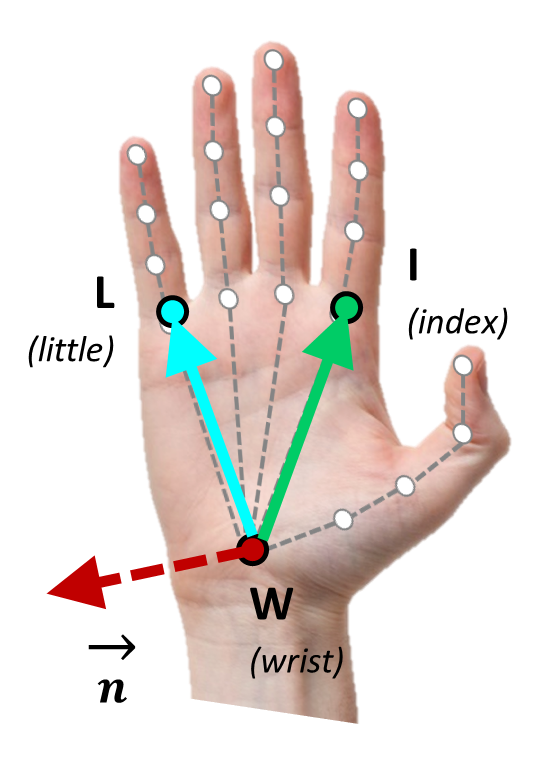
\includegraphics[height=3.8cm]{capitulos/metodos/imagens/palm_orientation_algebra}
                  }%
                  \hfill
                  \subcaptionbox{\label{subfig:palm-directions}}{
                      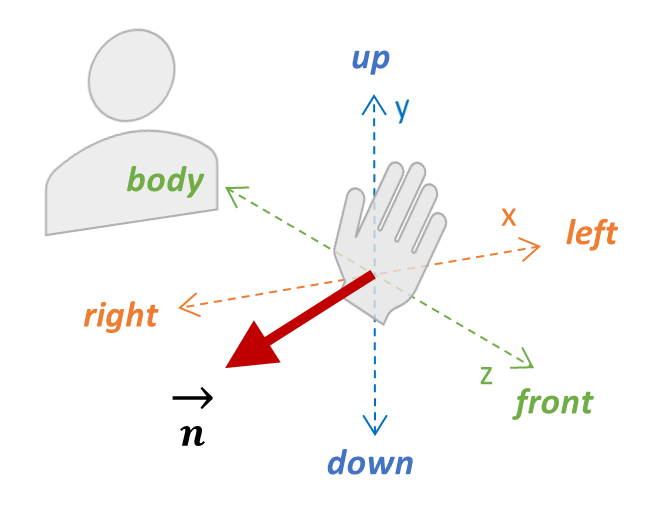
\includegraphics[height=4cm]{capitulos/metodos/imagens/hand_orientations}
                  }%
              }
              \nomefonte{}
              \label{fig:palm-orientation-directions}
          \end{figure}

          A partir dessas coordenadas, \citeonline{anton-2013-algebra} afirmam que pode-se estabelecer dois vetores auxiliares em termos dos quais esse mesmo plano cartesiano também é descrito (vide \autoref{subfig:palm-orientation}): \(\overrightarrow{WL}\), indicado pela seta azul e \(\overrightarrow{WI}\), indicado pela seta verde.
          Por meio deles, calculou-se o vetor normal \(\overrightarrow{n}\) utilizando a \autoref{eqn:normal-palm-left} (para a mão esquerda) e \autoref{eqn:normal-palm-right} (para a mão direita). \(\overrightarrow{n}\), que é perpendicular à palma da mão, é ilustrado na \autoref{subfig:palm-orientation} como uma seta tracejada vermelha.

          %   Por meio desses vetores deles, é possível estabelecer o vetor normal \(\overrightarrow{n}\) perpendicular ao plano da palma, que é indicado pela seta vermelha tracejada, e calculado conforme \autoref{eqn:normal-palm-left} (para a mão esquerda) e \autoref{eqn:normal-palm-right} (para a mão direita):

          % Palm orientation:
          \begin{equation}
              \label{eqn:normal-palm-left}
              \overrightarrow{n}_{left} = \overrightarrow{WI} \times \overrightarrow{WL}
          \end{equation}

          \begin{equation}
              \label{eqn:normal-palm-right}
              \overrightarrow{n}_{right} = \overrightarrow{WL} \times \overrightarrow{WI}
          \end{equation}

          Por fim, utilizou-se os valores das coordenadas de \(\overrightarrow{n}\) para definir a orientação da palma \(O_{palm}\), conforme \autoref{eqn:palm-orientation-directions}.
          Essa orientação consiste na combinação de até três das seguintes direções: \textit{right} (direita), \textit{left} (esquerda), \textit{up} (para cima), \textit{down} (para baixo), \textit{body} (voltada para o corpo) ou \textit{front} (para frente).
          Por exemplo, ``\textit{right\_front\_down}'' seria uma orientação válida indicando que a palma da mão está inclinada, conforme ilustrado na \autoref{subfig:palm-directions}.

          %   Finalmente, ao avaliar os valores dos eixos \(x\), \(y\) e \(z\) da normal \(\overrightarrow{n}\), é possível definir a orientação da palma \(O_{palm}\) como sendo a combinação de até três direções, cujas opções são: \textit{right} (direita), \textit{left} (esquerda), \textit{up} (para cima), \textit{down} (para baixo), \textit{body} (para o corpo) ou \textit{front} (para frente).
          %   Por exemplo, ``\textit{right\_down}'' e ``\textit{left\_up\_body}'' seriam orientações válidas. Essa avaliação é realizada conforme \autoref{eqn:palm-orientation-directions}:

          % Directions
          \begin{equation}
              \label{eqn:palm-orientation-directions}
              O_{palm} =
              \begin{cases}
                  right & \text{if $\overrightarrow{n}_x < {-k}$ } \\
                  left  & \text{if $\overrightarrow{n}_x > {k}$ }  \\
                  up    & \text{if $\overrightarrow{n}_y < {-k}$ } \\
                  down  & \text{if $\overrightarrow{n}_y > {k}$ }  \\
                  body  & \text{if $\overrightarrow{n}_z < {-k}$ } \\
                  front & \text{if $\overrightarrow{n}_z > {k}$ }  \\
              \end{cases}
          \end{equation}

          Na \autoref{eqn:palm-orientation-directions}, \(k\) é definido empiricamente como 0,30 para filtrar variações pouco significativas em \(\overrightarrow{n}\).


    \item \textbf{Movimento}: é o deslocamento realizado pelas mãos na articulação do sinal.

          Para calculá-lo, primeiro será selecionada como referência a coordenada \(M\) localizada na base do dedo médio (vide \autoref{subfig:hand-movement}).
          Em seguida, será obtido seu deslocamento entre os \textit{frames} anterior (tempo \(t-1\)) e atual (tempo \(t\)) utilizando a \autoref{eqn:hand-movement} que, por sua vez, fornecerá o vetor de movimento \(\overrightarrow{m}\) (indicado pela seta tracejada vermelha na \autoref{subfig:hand-movement}).

          \begin{figure}[ht!]
              \centering
              \caption{
                  \textmd{
                      O vetor de movimento \(\protect \overrightarrow{m}\) é obtido através da trajetória da coordenada \(M\) entre os frames anterior (\(t-1\)) e atual (\(t\))~(\subref{subfig:hand-movement}); \(\protect \overrightarrow{m}\) é então utilizado para calcular o movimento da mão \(V_{hand}\)~(\subref{subfig:hand-directions})
                      %   O movimento da mão \(V_{hand}\) é calculado a partir da trajetória da coordenada \(M\) entre os \textit{frames} anterior (\(t-1\)) e atual (\(t\))
                      %   O vetor de movimento \(\protect \overrightarrow{m}\) é calculado pela trajetória da coordenada \(M\) entre os frames anterior (\(t-1\)) e atual (\(t\))~(\subref{subfig:hand-movement}).
                      %   O movimento da mão \(V_{hand}\) é então obtido a partir de \(\protect \overrightarrow{m}\) e descrito dentre um conjunto de direções possíveis~(\subref{subfig:hand-directions}).
                  }
              }
              \borda[0.7\textwidth]{
                  \subcaptionbox{\label{subfig:hand-movement}}{
                      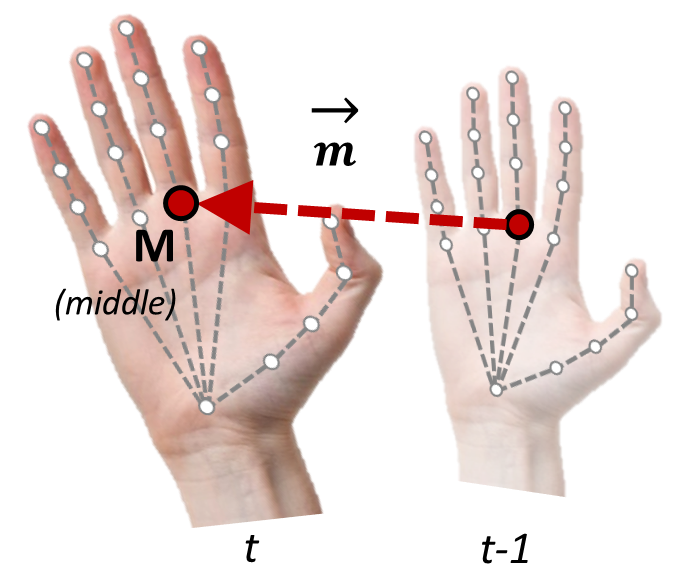
\includegraphics[height=3.5cm]{capitulos/metodos/imagens/hand_movement}
                  }%
                  \hfill
                  \subcaptionbox{\label{subfig:hand-directions}}{
                      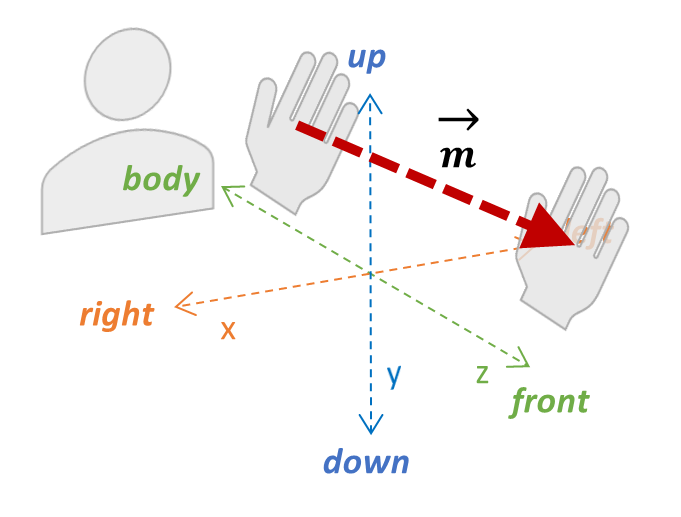
\includegraphics[height=4cm]{capitulos/metodos/imagens/hand_movement_2}
                  }%
              }
              \nomefonte{}
              \label{fig:hand-movement-directions}
          \end{figure}

          % Movement of the hands:
          \begin{equation}
              \label{eqn:hand-movement}
              \overrightarrow{m} = M_{t} - M_{t-1}
          \end{equation}

          A partir de \(\overrightarrow{m}\), pode-se então calcular o movimento da mão \(V_{hand}\) através da \autoref{eqn:hand-movement-directions}, que consiste numa operação semelhante àquela utilizada para a orientação da mão.
          Com isso, \(V_{hand}\) também consistirá na combinação de até três direções: \textit{right} (direita), \textit{left} (esquerda), \textit{up} (para cima), \textit{down} (para baixo), \textit{body} (para o corpo) ou \textit{front} (para frente).
          A \autoref{subfig:hand-directions} ilustra um movimento categorizado com a direção ``\textit{front}''.

          %   uma operação semelhante àquela utilizada para a orientação da mão, para definir o movimento da mão \(V_{hand}\) como a combinação de até três direções, cujas opções são: \textit{right} (direita), \textit{left} (esquerda), \textit{up} (para cima), \textit{down} (para baixo), \textit{body} (para o corpo) ou \textit{front} (para frente). Essa operação é detalhada na \autoref{eqn:hand-movement-directions} e a \autoref{subfig:hand-directions} ilustra ela segundo a perspectiva do sinalizador:

          % Directions
          \begin{equation}
              \label{eqn:hand-movement-directions}
              V_{hand} =
              \begin{cases}
                  right & \text{if $\overrightarrow{m}_x < {-k}$ } \\
                  left  & \text{if $\overrightarrow{m}_x > {k}$ }  \\
                  up    & \text{if $\overrightarrow{m}_y < {-k}$ } \\
                  down  & \text{if $\overrightarrow{m}_y > {k}$ }  \\
                  body  & \text{if $\overrightarrow{m}_z < {-k}$ } \\
                  front & \text{if $\overrightarrow{m}_z > {k}$ }  \\
              \end{cases}
          \end{equation}

          Na \autoref{eqn:hand-movement-directions} o limiar \(k\) foi também estabelecido empiricamente como 0,30, para filtrar movimentos com baixa relevância.


    \item \textbf{Expressão não-manual (abertura da boca)}: captura o grau de abertura da boca para cada \textit{frame} na articulação do sinal que, por sua vez, denota a existência de expressão não-manual envolvendo ela.

          Para computar essa \textit{feature}, utilizou-se como referência o trabalho de \citeonline{ferrario-2000-study-lips}, que analisa e propõe medidas antropométricas para os lábios.
          Dentre elas, foi selecionada a \textit{vermilion height to mouth width} (ou altura dos lábios com relação à largura da boca) para estabelecer a abertura da boca \(P_{mouth}\), uma vez que essa medida é capaz de capturar a proporção de abertura dos lábios em termos de um único número.
          A \autoref{eqn:mouth-openness} define formalmente o cálculo de \(P_{mouth}\), que consiste na proporção entre a altura e a largura dos lábios:

          % Abertura da boca:
          \begin{equation}
              \label{eqn:mouth-openness}
              P_{mouth} = \frac{d(LS, LI)}{d(CH_r, CH_l)}
          \end{equation}

          A altura dos lábios é dada pela distância \(d\) entre as coordenadas do \textit{labiale superius} \(LS\) e do \textit{labiale inferius} \(LI\), que são os pontos mais externos aos lábios superior e inferior, respectivamente. A largura, por sua vez, consiste na distância entre as coordenadas do \textit{cheilion} direito \(CH_r\) e do \textit{cheilion} esquerdo \(CH_l\), que são os pontos situados nos cantos direito e esquerdo dos lábios, conforme ilustra a \autoref{fig:mouth-openness}.

          \figura
          {fig:mouth-openness} % Label
          {capitulos/metodos/imagens/mouth_openness} % Path
          {height=3.5cm} % Size
          {A abertura da boca \(P_{mouth}\) é obtida a partir da medida antropométrica \textit{vermilion height to mouth width} que utiliza quatro coordenadas dos lábios para calcular uma única proporção} % Caption
          {ferrario-2000-study-lips} % Citation

\end{enumerate}


Essas são as \textit{features} extraídas para o ASL-Phono.
O \autoref{cod:sample-json-phono} exemplifica uma amostra resultante desse processo, bem como a disposição dos atributos fonológicos em suas propriedades.
Sua estrutura é muito semelhante àquela apresentada para o ASL-Skeleton3D, exceto pela propriedade ``\textit{frames}'' que, ao invés de coordenadas 3D, aqui contém os atributos computados acima. Além do seu respectivo valor computado, cada atributo pode apresentar também um \textit{score}, que é obtido a partir da precisão estimada para as coordenadas envolvidas no seu cálculo.

% \figura
% {fig:sample-json-phono} % Label
% {capitulos/metodos/imagens/code_phono} % Path
% {width=0.65\linewidth} % Size
% {Exemplo de amostra do ASL-Phono. Atributos com sufixo ``dh'' referem-se à \textit{dominant hand} (mão dominante) e aqueles com ``ndh'' referem-se à \textit{non-dominant hand} (mão não-dominante)} % Caption
% {} % Citation

\codigo
    {cod:sample-json-phono}
    {capitulos/metodos/codigos/exemplo_phono.m}
    {ASLDataset}
    {Exemplo de amostra do ASL-Phono: atributos com sufixo ``dh'' referem-se à \textit{dominant hand} (mão dominante) e aqueles com ``ndh'' referem-se à \textit{non-dominant hand} (mão não-dominante)}
    {}



% Estatísticas:
A \autoref{tab:dataset-phono-stats}, por sua vez, apresenta estatísticas calculadas para o \textit{dataset} resultante que nos fornecem um panorama da distribuição final de suas amostras, bem como do número de movimentos, orientações, configurações de mão e variação na abertura de boca computados acima.

% Na \autoref{tab:dataset-phono-stats}, podemos observar algumas estatísticas calculadas a partir do ASL-Phono, que nos permitem compreender como as amostras ficaram organizadas no \textit{dataset} após o processamento acima.

% Please add the following required packages to your document preamble:
% \usepackage{multirow}
% \usepackage{graphicx}
% \usepackage[table,xcdraw]{xcolor}
% If you use beamer only pass "xcolor=table" option, i.e. \documentclass[xcolor=table]{beamer}
\begin{table}[ht!]
    \centering
    \caption{Estatísticas calculadas a partir do ASL-Phono, as quais são visualizadas para todo o \textit{dataset} e segundo agrupamentos por amostra e por sinal. (D) refere-se à mão dominante e (ND) refere-se à mão não-dominante}
    \label{tab:dataset-phono-stats}
    \resizebox{0.9\textwidth}{!}{%
        \begin{tabular}{cr|ccc|ccccccc}
            \hline
            \rowcolor[HTML]{EFEFEF}
                                                                                     &        & \cellcolor[HTML]{EFEFEF}                           & \cellcolor[HTML]{EFEFEF}                         & \cellcolor[HTML]{EFEFEF}                         & \multicolumn{2}{c}{\cellcolor[HTML]{EFEFEF}Movimento} & \multicolumn{2}{c}{\cellcolor[HTML]{EFEFEF}Orientação} & \multicolumn{2}{c}{\cellcolor[HTML]{EFEFEF}Config. mão} & \cellcolor[HTML]{EFEFEF}                                                                                                                       \\
            \rowcolor[HTML]{EFEFEF}
                                                                                     &        & \multirow{-2}{*}{\cellcolor[HTML]{EFEFEF}Nº amostras} & \multirow{-2}{*}{\cellcolor[HTML]{EFEFEF}Nº sinais} & \multirow{-2}{*}{\cellcolor[HTML]{EFEFEF}Nº frames} & (D)                                                   & (ND)                                                   & (D)                                                     & (ND)                     & (D)  & (ND) & \multirow{-2}{*}{\cellcolor[HTML]{EFEFEF}\begin{tabular}[c]{@{}c@{}}Abertura \\ da boca\end{tabular}} \\ \hline
            \begin{tabular}[c]{@{}c@{}}\textit{Dataset}\end{tabular}      & Total  & 9.747                                              & 2.650                                            & -                                                & 26                                                    & 26                                                     & 26                                                      & 26                       & 85   & 78   & -                                                                                                     \\ \hline
                                                                                     & Mín    & -                                                  & -                                                & 1                                                & 0                                                     & 0                                                      & 0                                                       & 0                        & 0    & 0    & 0,01                                                                                                  \\
                                                                                     & Máx    & -                                                  & -                                                & 12                                               & 10                                                    & 8                                                      & 6                                                       & 5                        & 2    & 2    & 2,19                                                                                                  \\
                                                                                     & Média  & -                                                  & -                                                & 3,02                                             & 1,94                                                  & 1,26                                                   & 2,20                                                    & 1,18                     & 1,17 & 0,72 & 0,13                                                                                                  \\
            \multirow{-4}{*}{\begin{tabular}[c]{@{}c@{}}Por \\ amostra\end{tabular}} & Desvio & -                                                  & -                                                & 0,87                                             & 0,83                                                  & 1,15                                                   & 0,79                                                    & 1,07                     & 0,38 & 0,58 & 0,12                                                                                                  \\ \hline
                                                                                     & Mín    & 1                                                  & -                                                & -                                                & 1                                                     & 0                                                      & 1                                                       & 0                        & 1    & 0    & 0,02                                                                                                  \\
                                                                                     & Máx    & 59                                                 & -                                                & -                                                & 24                                                    & 16                                                     & 22                                                      & 14                       & 8    & 8    & 0,99                                                                                                  \\
                                                                                     & Média  & 3,68                                               & -                                                & -                                                & 6,04                                                  & 3,66                                                   & 5,37                                                    & 2,63                     & 1,81 & 1,17 & 0,13                                                                                                  \\
            \multirow{-4}{*}{\begin{tabular}[c]{@{}c@{}}Por \\ sinal\end{tabular}}   & Desvio & 2,67                                               & -                                                & -                                                & 2,93                                                  & 3,18                                                   & 2,29                                                    & 2,35                     & 0,99 & 1,14 & 0,07                                                                                                  \\ \hline
        \end{tabular}%
    }
    \nomefonte{}
\end{table}

Existem três agrupamentos contidos nessa tabela:

\begin{itemize}
    \item \textit{Dataset}: sumariza o total de amostras, de sinais e de cada um dos atributos computados para o \textit{dataset}.
          Por exemplo, há um total de 9.747 amostras e 26 movimentos possíveis para a mão dominante.

    \item Por amostra: fornece estatísticas de mínimo, máximo, média e desvio padrão calculadas agrupando-se o \textit{dataset} por amostra.
          Por exemplo, há em média 3,02 \textit{frames} por amostra e esse número varia de 1 a 12 \textit{frames}; de maneira semelhante, as amostras têm em média 1,94 movimentos distintos para a mão dominante, o que varia entre 0 e 10 movimentos.

          % contém estatísticas de números mínimos, máximos, médios e desvio padrão para os parâmetros computados acima. Por exemplo, lê-se que, em média, as amostras possuem 3,02 frames, sendo que a mais curta contém apenas 1 frame e a mais longa possui 12 frames. De maneira semelhante, as amostras têm em média de 1,94 movimentos e 2,20 orientações de mão distintas para a mão dominante.

    \item Por sinal: fornece estatísticas de mínimo, máximo, média e desvio padrão calculadas agrupado-se o \textit{dataset} por sinal.
          Por exemplo, cada sinal tem em média 3,68 amostras e isso pode variar de 1 até 59 -- no entanto, o desvio padrão nos revela que tal variação concentra-se muito mais em torno da média; nota-se também que a mão dominante realiza em média 6,04 movimentos distintos em um único sinal, o que pode variar de 1 a 24 para outros.

          % contém estatísticas de números mínimos, máximos, médios e desvio padrão para os sinais contidos no \textit{dataset}. Por exemplo, lê-se que cada sinal possui em média de 3,68 amostras, sendo que alguns deles possuem apenas 1 e outros possuem valores atípicos de 59 amostras (a considerar pelo desvio padrão apresentado). Além disso, cada sinal apresenta em média 6,04 movimentos e 5,37 orientações de mão distintas para a mão dominante.
\end{itemize}


Por fim, a \autoref{fig:dataset-resampling-antes} detalha a relação entre o número de sinais e o número de amostras existentes no ASL-Phono. Por meio desta análise, percebe-se mais claramente que a maior parte dos sinais concentra-se na faixa de 1 e 6 amostras, que é exatamente o intervalo descrito pela média e desvio padrão da tabela acima.
No entanto, há sinais que apresentam 7 ou mais amostras e ainda outros casos atípicos em que 1, 2 ou 3 sinais que concentram sozinhos um número muito grande de amostras -- de 13 até 59.
Será discutida na seção seguinte a abordagem utilizada neste trabalho para lidar com esse desbalanceamento e homogeneizar as amostras antes de prosseguir com os experimentos.

\figura
{fig:dataset-resampling-antes} % Label
{capitulos/metodos/imagens/dataset_resampling_antes} % Path
{height=5.5cm} % Size
{Relação entre número de sinais e número de amostras disponíveis no ASL-Phono} % Caption
{} % Citation


O \textit{dataset} e o código-fonte resultantes do processamento apresentado nesta seção estão disponíveis publicamente na URL listada abaixo\footnote{Disponível em \url{http://www.cin.ufpe.br/~cca5/asl-phono}}.
